
\documentclass[a4paper,12pt]{article}
\usepackage[french]{babel}  % Langue française
\usepackage[T1]{fontenc}    % Encodage des caractères
\usepackage[utf8]{inputenc} % Encodage UTF-8
\usepackage{graphicx}       % Pour insérer des images
\usepackage{amsmath, amssymb} % Mathématiques
\usepackage{hyperref}       % Liens hypertextes
\usepackage{geometry}       % Mise en page
\usepackage{verbatim}
\geometry{margin=2.5cm}    % Marges

\begin{document}

% Page de titre
\title{\textbf{projet stats app séance du 16/04/25}}
\maketitle

% Résumé
%\begin{abstract}
%\end{abstract}

% Introduction
\section{Introduction}

La méthode de double différence appliquée à la variation de la zone inondable en 2020 n’ayant pas donné de résultats concluants, nous avons cherché à l’appliquer à un autre événement : l’inondation majeure survenue dans l’Aude en octobre 2018. Lors de cet épisode, les hauteurs d’eau ont atteint, à certains endroits, des niveaux jamais enregistrés depuis 1891. En plus des importants dégâts matériels, l’inondation a causé la mort de 15 personnes et blessé 99 autres. Au total, 257 communes ont été rapidement reconnues en état de catastrophe naturelle, dont 204 dans l’Aude, 29 dans l’Hérault et 24 dans le Tarn. \newline

\begin{figure}[ht]
    \centering
    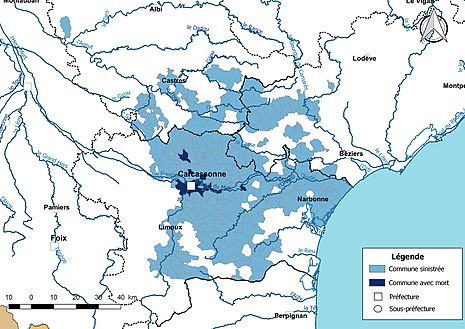
\includegraphics[width=0.8\textwidth]{Crue-oct18-Catnat.jpg}
    \caption{Communes sinistrées déclarées en état de catastrophe naturelle}
    \label{fig:mon_image}
\end{figure}

Pour appliquer la méthode des doubles différences, nous avons restreint notre analyse à un groupe de communes situées autour du Carcassonnais, zone particulièrement touchée par l’inondation. Le groupe de traitement comprend une cinquantaine de communes, incluant toutes celles où des décès ont été recensés. Le groupe de contrôle, quant à lui, est composé d’environ 70 communes situées à l’ouest de Carcassonne. Ces dernières n’ont pas été déclarées en état de catastrophe naturelle, mais sont suffisamment proches géographiquement pour être considérées comparables. Cette sélection vise à satisfaire l’hypothèse de tendance parallèle entre les deux groupes. \newline

Nous avons par ailleurs considéré uniquement les transactions dans une fenêtre d'un an avant et un an après l'inondation.\newline

Ci-dessous, le nombre de transactions suivant la zone de rsique et l'année: 
\begin{itemize}
\item nombre d'observations: 1473
\item nombre de transactions dans le groupe traité: 960
\item nombre de transaction dans le groupe de contrôle: 513
\item nombre de transactions après l'inondation: 589
\item nombre de transactions avant l'inondation: 371
\item nombre de transactions $traitement\_post = 1$: 369
\end{itemize}


% Modèle et Méthodologie
\section{Modèle}
Nous utilisons la régression linéaire suivante :
\begin{equation}
	\log(\text{prix/m}^2_{it}) = \beta_0 + \beta_1 \times \text{Traitement} + \beta_2 \times \text{Post} + \beta_3 \times \text{Post} \times \text{Traitement} + controles + \varepsilon
\end{equation}

Où Traitement représente une variable binaire pour l'appartenance au groupe de traitement. Post est aussi une variable binaire valant 1 pour une date de mutation supérieure au 15 octobre 2018 dans la limite d'un an et 0 pour une date de mutation inférieure au 15 octobre 2018 dans une limite d'un an. \newline

Les contrôles sont les suivants:
\begin{itemize}
\item distance à la mairie
\item distance au littoral
\item distance au fleuve
\item nombre de dépendances (variables indicatrices de 1 à 3)
\item nombre de pièces principales (variables indicatrices de 1 à 6)
\item surface batie
\item surface terrain
\item prix moyen dans la ville
\end{itemize}

% Résultats
\section{Résultats}

Ci-dessous, les résultats de la différence de différence. \newline

\verbatiminput{resultat_DID_Aude.txt}

% Conclusion
\section{limites}
\begin{itemize}
\item coefficient causal non significatif
\item TODO: réduire le nombre de communes dans le groupe de traitement
\item double différence avec effets fixes ?
\end{itemize}

\end{document}
